\label{ch:desing}
\chapter{Diseño e Implementación}

\section{Limitaciones técnicas para implementar el prototipo}

\section{Diseño de la solución} 
Definición Política de seguridad:\newline
Detectar si una aplicación android(características conjunto de evaluación)
presenta flujos de información entre, información con niveles de seguridad alto
e información con nivel de seguridad bajo.\newline Detectando fugas de
información catalogada con nivel de seguridad alto, vía: canales creados durante
el control de flujo del programa(flujos implicitos), mensajes de texto y
mensajes de Log. \newline
El conjunto de aplicaciones a evaluar se caracteriza por:\newline
extender de una de las siguientes clases de la API de Android: Activity,
BroadcastReceiver o Service. En otras palabras, aplicaciones con un único punto
de entrada. \newline 
enviar información a través de las siguientes clases de la
API de Android: Log y SmsManager.\newline



Cómo verificar el cumplimiento de está política mediante
Jif?
\newline \begin{figure}[h!]
	\begin{center}
	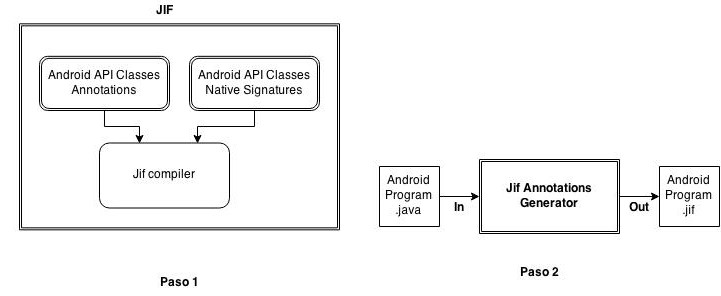
\includegraphics[width=12cm]{desingSol-steps1-2.jpg}
	\end{center}
	\caption{Pasos para el diseño de la solución.}
	\label{fig:desingSol-steps1-2}
\end{figure}

Paso uno: hacer que jif reconozca determinadas clases de la Api de
Android\newline 

\begin{figure}[h!]
	\begin{center}
	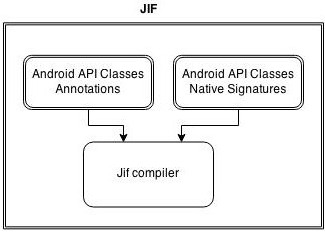
\includegraphics[width=5cm]{desingSol-step1.jpg}
	\end{center}
	\caption{Diseño de la solución paso 1. Ilustra dos tipos de anotaciones que
	deben ser incluidas para que el compilador reconozca clases de la API de
	Android.}
	\label{fig:desingSol-step1}
\end{figure}

Paso dos: 
Definir Autoridades y forma de annotación del programa android a analizar.
Una clase Android tendrá una Autoridad máxima(un principal), en este caso Alice,
así que, información con nivel de seguridad alto deberá pertenecer a dicha
autoridad.\newline
Jif hace seguimiento al flujo de información del programa, asociando un label
de seguridad al program counter de cada sentencia y expresion del programa,
program counter(pc) label. Este pc se ve afectado por el label
de seguridad que se especifique en la declaración de variables y
métodos.\newline 
La sintaxis para anotación de variables es: \newline 
\emph{ type\{L\} varName; } \newline donde type especifíca el tipo de dato que
almacena la variable, \{L\} el label de seguridad  para especificar quien es el
dueño de la variable, y name, el respectivo nombre de la variable.\newline 
Un método se escribe de la forma:\newline
\emph{ type \{RTL\} methodName \{BL\} (arg1\{AL\},,, argn\{AL\}) :\{EL\}
}\newline RTL, Return Type Label, indica el label de seguridad con que
queda el tipo de dato devuelto por el método.\newline 
BL begin label, representa el máximo nivel se seguridad del pc label desde donde
se invoca el método, de este modo, el program counter label desde donde
se invoca el método debe ser menor o igual de restrictivo que el BL del
método.\newline 
AL argument label, indica el máximo nivel de seguridad de los argumentos con que
se invoca el método, así, los labels de los argumentos con que se invoca el
método deben ser menor o igual de restrictivos que los AL con que han
definido el método.\newline
EL end label, indica el pc label en el punto de terminación del método, y
representa la información que puede ser conocida.\newline
Cuando un label no es específicado, Jif define unos por defecto. En el caso de
RTL, jif hace un join entre los diferentes AL con que ha sido definido el
método.\newline

Partiendo de que Jif se fundamenta en labels de seguridad para hacer seguimiento
al flujo de información del programa, es necesario definir los labels a
anotar para métodos y variables del programa.\newline
En el caso de variables con nivel de seguridad  alto, la anotación debe
ser:\newline
\emph{ type\{Alice:\} varName; }\newline
Para el resto de variables, entran a jugar las anotaciones definidas por Jif
acorde al contexto donde están definidas.

Ahora en el caso de los métodos, la anotación varía acorde a si el método debe
influenciar(acceder, modificar) o no, información anotada con nivel de seguridad
alto.
Partiendo de lo anterior, se define un algoritmo de anotación que se condensa en
un generador de anotaciones\newline
\begin{figure}[h!]
	\begin{center}
	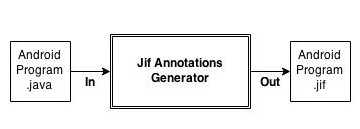
\includegraphics[width=6cm]{desingSol-step2.jpg}
	\end{center}
	\caption{Diseño de la solución paso 2. Ilustra salidas y entradas del
	generador de anotaciones.}
	\label{fig:desingSol-step1}
\end{figure}




